\documentclass{article}


\usepackage[14pt]{extsizes}
\usepackage[top=20mm, bottom=20mm, left=30mm, right=10mm, paperwidth=210mm, paperheight=297mm]{geometry}
\usepackage{amsmath,amsthm,amssymb}
\usepackage{mathtext}
\usepackage{cmap}
\usepackage[T1,T2A]{fontenc}
\usepackage[utf8]{inputenc}
\usepackage[russian]{babel}
\usepackage{graphicx,subcaption,caption,float}
\usepackage{fancyhdr}
\usepackage{listings}
\usepackage{multirow}
\usepackage{color}
\usepackage{indentfirst}
\usepackage{tabulary}

%% Setting up packages

% listings
\definecolor{colorSourceComment}{rgb}{0,0.6,0}
\definecolor{colorSourceString}{rgb}{0.58,0,0.82}

\lstset{
  basicstyle=\footnotesize\sffamily,
  breaklines=true,
  captionpos=t,
  commentstyle=\color{colorSourceComment},
  frame=l,
  keepspaces=true,
  keywordstyle=\color{blue},
  numbers=left,
  numbersep=5pt,
  numberstyle=\footnotesize\sffamily,
  % showstringspaces=false, %%
  stringstyle=\color{colorSourceString},
  tabsize=2,
  title=\lstname
}

% fancyhdr
\renewcommand{\headrulewidth}{0pt}

\newcommand{\Section}[1]
{
  \newpage
  \section{#1}
}

\newcommand{\Sectionx}[1]
{
  \newpage
  \section*{#1}
  \addcontentsline{toc}{section}{#1}
}

\newcommand{\ssection}[1]{\subsection{#1}}
\newcommand{\sssection}[1]{\subsubsection{#1}}
\renewcommand\labelitemi{---}

%% Setting up document info
\title{Test}
\author{RubyScorp}
\date{\today}

\begin{document}
\section{Введение}
Игровые приложения представляют собой совершенно особый тип программ. Некоторые игры можно считать своеобразными произведениями искусства, в которых пользователь одновременно выступает в качестве актера и режиссера. Разработка интерфейсов игровых программ предполагает не только решение сугубо утилитарных задач, связанных с обеспечением простоты и удобства управления игрой, но еще и создание у пользователя определенного эмоционального настроя.

\bigskip\noindent Хорошая игра должна,
\begin{itemize}
  \item во-первых, \text{увлекать и всецело затягивать},
  \item во-вторых -- \text{вызывать чувство эстетического удовлетворения}.
\end{itemize}

\textbf{Цель -- удовлетворение пользователя}

Компьютерная эргономика и эргономика компьютерных игр имеют одинаковую цель: адаптировать приложение для использования конкретным человеком в конкретной ситуации. Для того, чтобы сделать приложение действительно удобным в использовании, необходимо знать, для каких целей оно будет применяться. Если речь идет о компьютерных играх, то их целью является развлечение, получение удовольствия.

Задачей эргономики является создание оптимальных условий труда, создающих у человека чувство удовлетворения от проделанной работы. При работе с программным обеспечением чувство удовлетворения возникает, если пользователь успешно и без лишних усилий выполняет с помощью программы ту или иную задачу. Компьютерные игры являются весьма специфическим видом ПО, в котором удовлетворение пользователя обусловлено целым рядом специфических факторов.

\section{Факторы, влияющие на удовлетворение пользователя игрового ПО}
Анализируя особенности юзабилити компьютерных игр, необходимо принимать во внимание специфику игрового опыта. К числу наиболее важных для пользователя характеристик игрового ПО относятся следующие:

\subsection{Простота использования}
Данный критерий принадлежит к числу решающих при оценке пользователями любой компьютерной программы. В случае с играми простота очень тесно связана с легкостью овладения. Не следует забывать и о понятности интерфейса, а также о легкости использования периферийных устройств.

\textbf{Начало игры} -- Меню, с помощью которого осуществляется запуск игры, следует уделять особое внимание. Разработчик должен быть уверенным в том, что:
\begin{itemize}
  \item пользователь получил исчерпывающую информацию о возможностях игры;
  \item после ознакомления с меню пользователь может управлять игровым процессом без проблем
\end{itemize}

\textbf{Обучающие уровни} -- Если игра включает обучающие уровни, то они должны быть органичной ее частью. Они должны отвечать следующим требованиям:
\begin{itemize}
  \item не быть как слишком трудными, так и слишком легкими;
  \item после прохождения обучающих уровней у пользователя должно возникнуть желание продолжать игру
\end{itemize}

\textbf{Игровой интерфейс} -- Его задачей является обеспечение обратной связи с пользователем, а также осуществление некоторых действий. К игровым интерфейсам применяются такие же требования, как и к интерфейсу любого ПО.

\textbf{Управление игрой с помощью периферийных устройств} -- Управление любой периферией должно осуществляться <<на автомате>>. Выбор кнопок и их функции должны быть обусловлены исключительно удобством пользователя.

\bigskip

Элементы, не относящиеся собственно к игре, не должны отвлекать пользователя от игрового процесса. Меню, сохранение уровней и т. п. -- все это должно быть предельно простым и не занимать большую часть внимания пользователя. Впрочем, в некоторых случаях бывает необходимо руководствоваться не столько критериями удобства, сколько эстетики. Визуально привлекательный интерфейс, анимация, выполняющая исключительно декоративные функции, необычное оформление меню -- все это может способствовать погружению, затягиванию пользователя в игру и тем самым повышать степень его удовлетворенности.

\bigskip

\noindent\textit{Рекомендации:}
\begin{itemize}
  \item \textit{Избегайте продолжительных вступлений}. Вместо того чтобы начинать игру с закадрового голоса, видеозаставки или титров, сразу передайте игроку активное управление. Задавайте сцену не словами, а настроением и атмосферой. Пусть о новых персонажах рассказывают их действия, а не биографии.
  \item \textit{Старайтесь как можно органичнее встраивать индикаторы в игровое окружение}. Например, разместите индикатор количества патронов в виде экрана непосредственно на самом оружии. Или сделайте такую систему инвентаря, которая существовала бы в физическом пространстве -- внутри рюкзака пользователя -- а не просто в меню на экране.
  \item \textit{Используйте модели повреждения или другие уникальные контекстуальные решения вместо индикаторов здоровья}. Например, о низком уровне здоровья противника могут свидетельствовать его медленная походка или хромота.
  \item \textit{Используйте простую контекстно зависимую систему управления вместо сложной и обширной}. Если ваш игрок может открывать сундуки и двери, значит оба действия должны выполняться одной кнопкой. Остается лишь позаботиться о том, чтобы двери и сундуки не попадались рядом.
  \item Говоря о контекстно зависимой системе, одну и ту же кнопку можно нажать несколькими разными способами: одинарное нажатие, двойное нажатие, нажатие с удержанием или серия ритмичных нажатий. Может возникнуть желание воспользоваться всеми возможностями контроллера, но постарайтесь найти способ ограничить количество нажимаемых кнопок до строго необходимого.
\end{itemize}

\subsection{Ритм игры}
Здесь речь идет обо всем, что способствует <<затягиванию>> пользователя в игровой процесс, и в первую очередь -- об интерактивности и о сюжете игры.

\textbf{Интерактивность} -- Смысл интерактивности заключается в создании у пользователя уверенности в том, что он управляет всем игровым процессом

\textbf{Сюжет} -- Хорошо продуманный сюжет позволяет увеличить степень интеграции пользователя в игровой процесс. Отношения между персонажами игры и пользователем, а также их смысловой контекст являются в данном случае главными факторами.

\noindent\textit{Рекомендации:}
\begin{itemize}
  \item \textit{Дайте вашим игрокам повод не нажимать на кнопку}. Если ожесточенная пальба в коридоре представляется оптимальным решением для одной ситуации, то отсутствие стрельбы может стать неплохим решением для другой. Вместо того, чтобы постоянно добавлять новые механики, подумайте о том, чтобы временно убрать существующие. Возможно, это принесет вашим игрокам новые ощущения.
  \item \textit{Больше исследований, меньше объяснений}. Не заваливайте игроков тоннами текста с предысторией и практическими советами, лучше вознаграждайте их за самостоятельное исследование игрового мира.
  \item \textit{Избегайте дополнительных предметов коллекций, объясняющих важные моменты из истории вашего игрового мира}. Найдите способ выразить эту информацию через геймплей, а не, скажем, аудиовставки.
  \item \textit{Молчание может быть не менее содержательным, чем полноценный диалог}. По возможности используйте язык тела и выражения лица для передачи эмоций.
  \item \textit{Заставляйте игрока ставить вопросы и не бойтесь оставлять их без ответа}. Игра, любой аспект которой открыт для познания и исследования, всегда будет иметь ограниченную глубину. Тайны и загадки, не подвластные изучению, надолго останутся в памяти игроков даже после завершения игры.
  \item \textit{Очень простой сюжет можно компенсировать, выдвинув на первый план сложный процесс совершенствования игрока}. Создание подобного контраста между двумя элементами, может вызвать у игрока ложное ощущение глубины.
\end{itemize}

\subsection{Степень трудности игры}
Степень трудности игры является одним из важных факторов, определяющих ее успешность. Игровой процесс должен быть организован так, чтобы задачи, возникающие перед пользователем, были достаточно сложными и чтобы их сам процесс их решения был приятен, интересен для пользователя. Уровень трудности игры должен соответствовать уровню пользовательской компетенции.

\textbf{Сложность} -- Уровень сложности игры должен быть обусловлен в первую очередь уровнем компетенции пользователя. По мере освоения пользователем специфики игры должны становиться более сложными и решаемые задачи.

\textbf{Тип задачи} -- Тип решаемых задач также очень важен: так, в автомобильных гонках пользователь должен не угадывать, в какую сторону повернет автомобиль после нажатия той или иной кнопки, но научиться управлять автомобилем. Специфика игровых задач должна соответствовать общему контексту игры и отвечать ожиданиям пользователя.

\textbf{Возможность компенсации} -- Пользователь игрового приложения в отличие от пользователя офисного ПО является мотивированным исследователем. Зачастую на решение той или иной задачи затрачивается немало времени и сил. Организация игрового процесса должна предусматривать возможность компенсации усилий, направленных на преодоление трудностей.

\bigskip

Перечисленные выше критерии основаны на рекомендациях группы по тестированию компьютерных игр компании Microsoft. Учет этих критериев позволяет существенно улучшить игру и максимально приблизить ее к ожиданиям пользователя.

\bigskip

\noindent\textit{Рекомендации:}
\begin{itemize}
  \item \textit{Всегда отдавайте предпочтение чему-либо знакомому, а не уникальному}. Звучит крайне неэффективно для любого, кто стремится изобретать что-нибудь новое, но это правда. Если вы создаете что-то, что каким-либо образом пересекается с уже существующими вещами, игроки легче освоятся в игре. Не стоит заново изобретать велосипед для того, кто уже умеет крутить педали.
  \item \textit{Используйте при построении головоломок и испытаний возможности ритма и синхронности}. Игроки быстро воспринимают подобные паттерны геймплея, не нуждаясь при этом в дополнительных инструкциях и объяснениях.
  \item \textit{Принуждайте игроков, открывших новую способность, самостоятельно упражняться и экспериментировать с ней}. Нет никакой необходимости в описаниях и обучающих уроках, просто заставьте игрока применить новую способность для решения немедленно возникшей задачи. Затем вам необходимо будет позаботиться о том, чтобы эта способность оставалась актуальной на протяжении всей игры, иначе она просто забудется.
  \item \textit{Нет излишествам}. Как правило, обилие вариантов – это хорошо, но убедитесь, что наиболее предпочтительный вариант не сводит на нет актуальность некоторых других вариантов. К примеру, если в игре есть реактивный ранец, бонусы в виде двойных прыжков или альпинистского крюка автоматически станут ненужными. Когда одно решение очевидным образом превосходит все остальные варианты, последние неизменно превращаются в излишество. Если у вас в игре есть много вариантов чего-либо, позаботьтесь о том, чтобы каждый из них давал уникальный и ценный бонус.
\end{itemize}

\section{Методы уничтожения игровых интерфейсов}
\subsection{Хороший интерфейс}
В проектировании игр и интерфейсов много общего. Более того, их можно рассматривать как вещи одного порядка, объединяемые более общей категорией -- проектированием опыта взаимодействия (UX design). В этом случае разница между ними следующая: процесс создания игры -- это проектирование игрового опыта (ощущений, эмоций), а создание интерфейса -- это проектирование опыта его использования (сценариев решения задач).

\begin{figure}[H]
  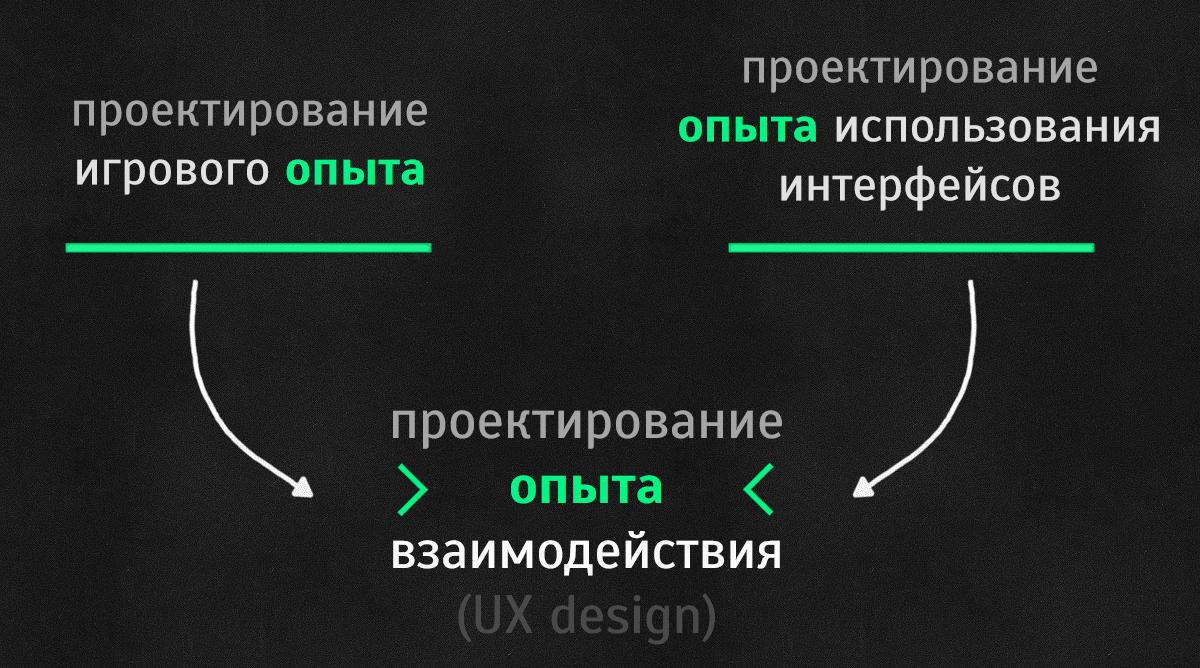
\includegraphics[width=\textwidth]{res/img/uxDesign.png}
  \caption{UX design}
\end{figure}

Существуют различные игровые механики, которые в совокупности с контентом формируют опыт игрока, начиная от элементарных и даже инстинктивных реакций, заканчивая сложными эмоциями.

Грубо говоря: раннеры создают чувство скорости и соперничества, хорроры вызывают страх, а сюжетные игры имеют потенциал передать любую эмоцию через историю, и так далее. Дизайн каждого ощущения и каждой эмоции при этом специфичен.

В случае же с интерфейсами, проектируемый опыт всегда имеет одно ключевое направление -- \textbf{ясность взаимодействия}. Абсолютно любой интерфейс должен обеспечивать удобство использования, а достигается это универсальными методами, о которых далее.

\begin{figure}[H]
  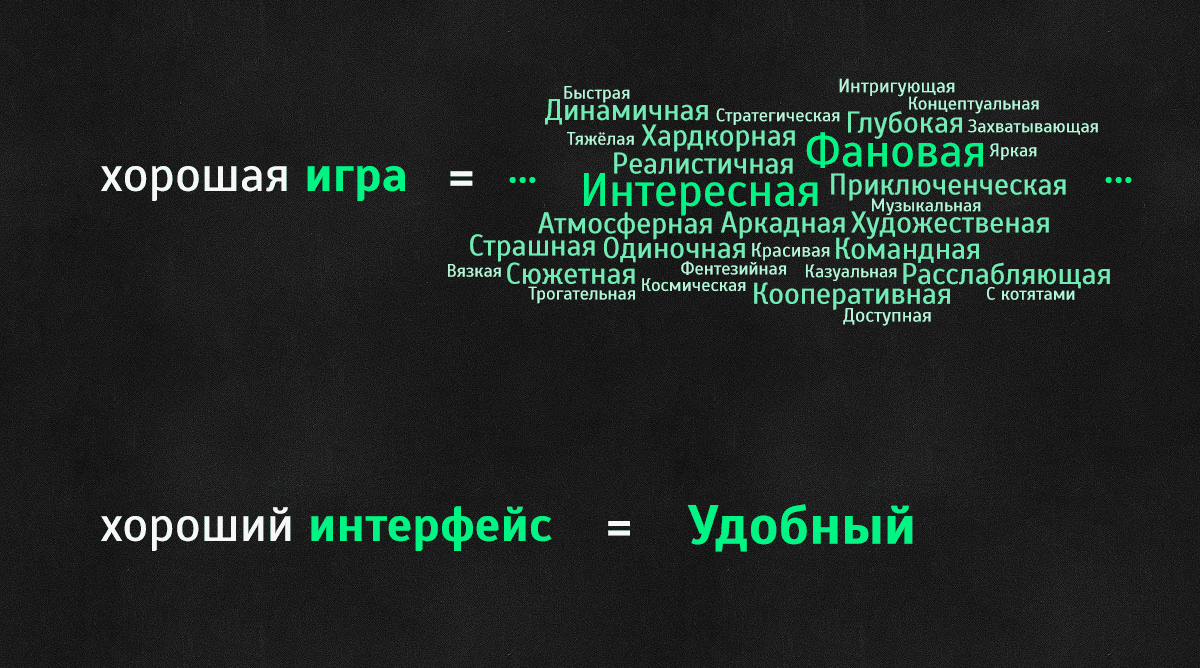
\includegraphics[width=\textwidth]{res/img/goodGame.png}
  \caption{Хорошая игра/Удобный интерфейс}
\end{figure}

\textit{Цель любого интерфейса – помочь пользователю решить конкретную задачу.}

Очень здорово, когда интерфейс не только \textit{помогает решить проблему}, но и \textit{ощущается максимально комфортно для пользователя} -- когнитивное и физическое сопротивление при его использовании стремится к нулю.

\bigskip

\noindent\textit{Любой хороший интерфейс должен быть:}
\begin{itemize}
  \item \textit{Понятным}. В любой момент времени пользователь интерфейса понимает, как взаимодействовать с ним для решения своей проблемы.
  \item \textit{Эффективным}. Интерфейс ведет пользователя по оптимальному пути решения его проблемы.
\end{itemize}

\subsection{Как добиться такого результата?}
В общем-то, в этом и заключается работа UX/UI-специалистов. Давайте перейдем к практике и познакомимся с их методиками поближе. Как диагностировать нездоровье ваших интерфейсов? Самый надежный и интересный способ -- \textbf{плейтесты} (хотя в данном случае это скорее юзабилити-тестирование). Отмечайте любые моменты, когда игроки (пользователи) <<зависают>>, хотя бы на пару секунд. Скорее всего, они растеряны или в чем-то сомневаются.

Попросите игроков обозначать вслух каждый раз, когда они не понимают, что от них требуется, как именно они должны действовать, или когда результат их действий расходится с ожиданиями.

Подсказками, указывающими на конкретные (и, к счастью, решаемые) проблемы, являются вопросы игроков вроде:
\begin{itemize}
  \item Как я могу сделать это?
  \item Что я должен сделать сейчас?
  \item Что произойдет, когда я сделаю это?
  \item Этот элемент интерактивен?
  \item Почему что-то изменилось, когда я ничего не делал?
  \item Как именно я должен это понимать/использовать?
\end{itemize}

Хорошо, допустим, проблемные места найдены. Но как именно сделать интерфейс понятным?

Для начала нужно составить лист задач, которые пользователь решает с помощью ваших интерфейсов. Начиная от внешних для геймплея: <<Запустить игру>>, <<Настроить>>, <<Выйти из игры>> -- заканчивая любыми внутриигровыми (геймплейными) взаимодействиями -- <<Двигаться>>, <<Использовать способность>>, <<Контролировать ресурсы>> -- их может быть бесконечно много и они могут быть сколь угодно разными. Тут все очень индивидуально и зависит от конкретной игровой механики. Кстати, иногда внешние задачи решаются через геймплейные интерфейсы, и это положительно сказывается на вовлеченности игрока.

\subsection{Примеры интерфейсов}
\subsubsection*{Геймплейный интерфейс}
 При запуске, Braid встречает игрока нестандартным стартовым экраном, а выбор уровня представляет из себя тот же игровой интерфейс -- перемещение персонажа по комнатам.

\begin{figure}[H]
  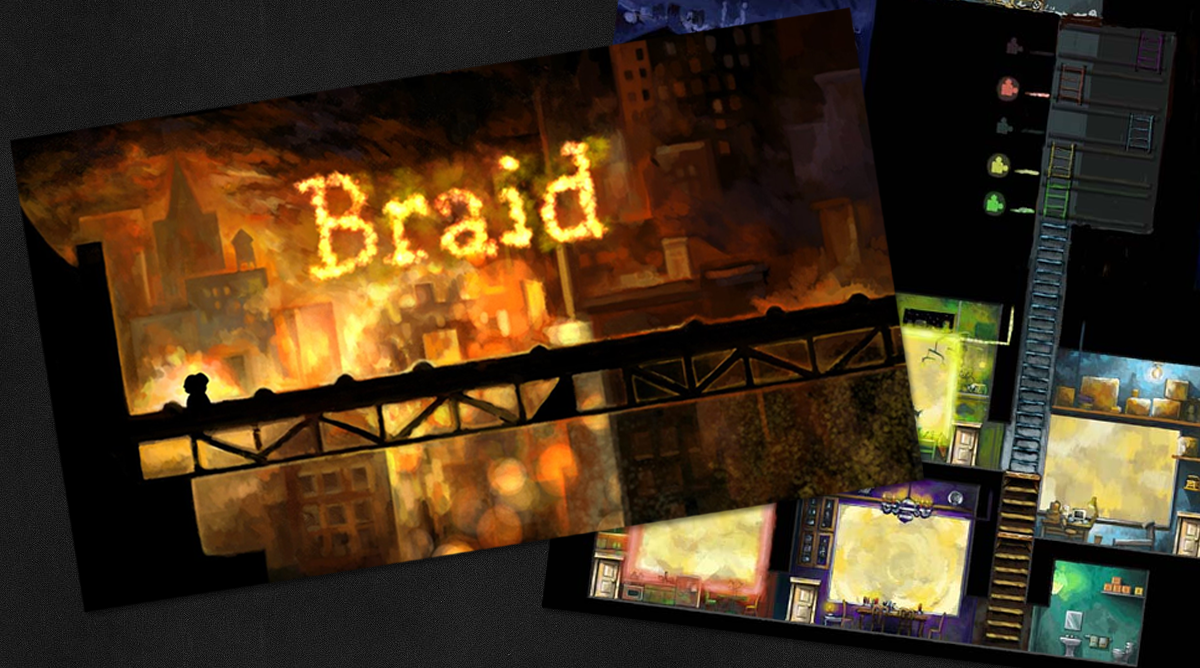
\includegraphics[width=\textwidth]{res/img/braid.png}
  \caption{Геймплейный интерфейс. Braid}
\end{figure}

Еще один хороший пример -- Fruit Ninja, который с главного меню знакомит игрока с базовой механикой.

\begin{figure}[H]
  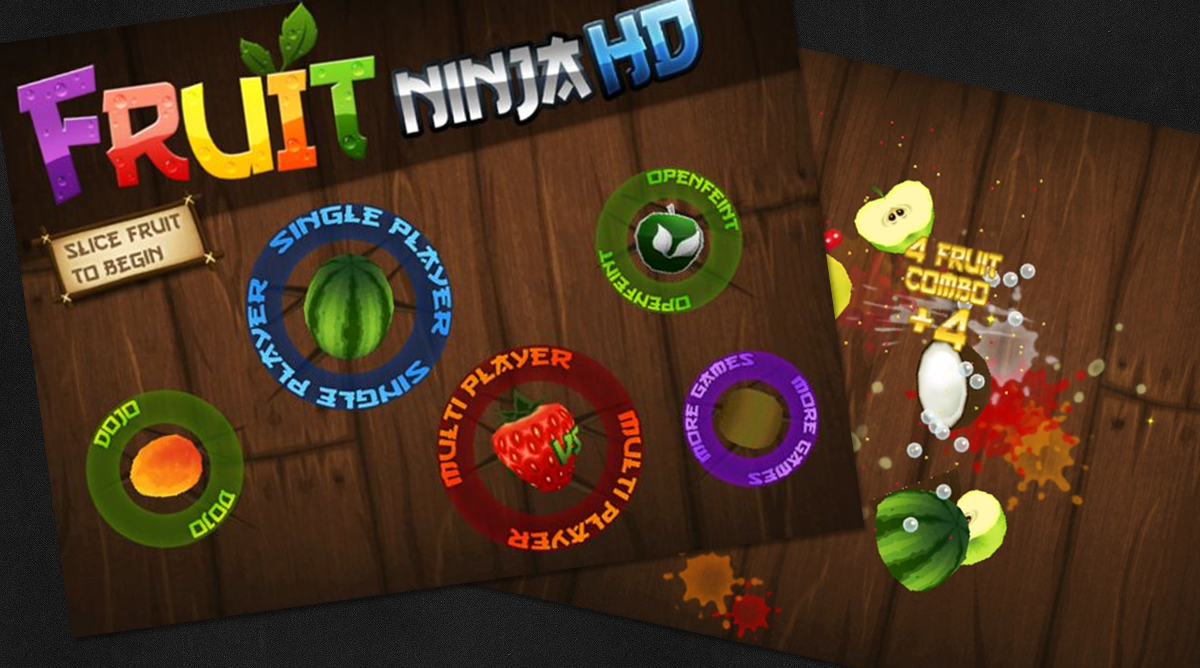
\includegraphics[width=\textwidth]{res/img/fruitNinja.png}
  \caption{Геймплейный интерфейс. FruitNinja}
\end{figure}

\subsubsection*{Классическоий интерфейс}

\end{document}
